
%% bare_conf_compsoc.tex
%% V1.4b
%% 2015/08/26
%% by Michael Shell
%% See:
%% http://www.michaelshell.org/
%% for current contact information.
%%
%% This is a skeleton file demonstrating the use of IEEEtran.cls
%% (requires IEEEtran.cls version 1.8b or later) with an IEEE Computer
%% Society conference paper.
%%
%% Support sites:
%% http://www.michaelshell.org/tex/ieeetran/
%% http://www.ctan.org/pkg/ieeetran
%% and
%% http://www.ieee.org/

%%*************************************************************************
%% Legal Notice:
%% This code is offered as-is without any warranty either expressed or
%% implied; without even the implied warranty of MERCHANTABILITY or
%% FITNESS FOR A PARTICULAR PURPOSE! 
%% User assumes all risk.
%% In no event shall the IEEE or any contributor to this code be liable for
%% any damages or losses, including, but not limited to, incidental,
%% consequential, or any other damages, resulting from the use or misuse
%% of any information contained here.
%%
%% All comments are the opinions of their respective authors and are not
%% necessarily endorsed by the IEEE.
%%
%% This work is distributed under the LaTeX Project Public License (LPPL)
%% ( http://www.latex-project.org/ ) version 1.3, and may be freely used,
%% distributed and modified. A copy of the LPPL, version 1.3, is included
%% in the base LaTeX documentation of all distributions of LaTeX released
%% 2003/12/01 or later.
%% Retain all contribution notices and credits.
%% ** Modified files should be clearly indicated as such, including  **
%% ** renaming them and changing author support contact information. **
%%*************************************************************************


% *** Authors should verify (and, if needed, correct) their LaTeX system  ***
% *** with the testflow diagnostic prior to trusting their LaTeX platform ***
% *** with production work. The IEEE's font choices and paper sizes can   ***
% *** trigger bugs that do not appear when using other class files.       ***                          ***
% The testflow support page is at:
% http://www.michaelshell.org/tex/testflow/



\documentclass[conference,compsoc]{IEEEtran}
% Some/most Computer Society conferences require the compsoc mode option,
% but others may want the standard conference format.
%
% If IEEEtran.cls has not been installed into the LaTeX system files,
% manually specify the path to it like:
% \documentclass[conference,compsoc]{../sty/IEEEtran}





% Some very useful LaTeX packages include:
% (uncomment the ones you want to load)


% *** MISC UTILITY PACKAGES ***
%
%\usepackage{ifpdf}
% Heiko Oberdiek's ifpdf.sty is very useful if you need conditional
% compilation based on whether the output is pdf or dvi.
% usage:
% \ifpdf
%   % pdf code
% \else
%   % dvi code
% \fi
% The latest version of ifpdf.sty can be obtained from:
% http://www.ctan.org/pkg/ifpdf
% Also, note that IEEEtran.cls V1.7 and later provides a builtin
% \ifCLASSINFOpdf conditional that works the same way.
% When switching from latex to pdflatex and vice-versa, the compiler may
% have to be run twice to clear warning/error messages.



\usepackage{graphicx}


% *** CITATION PACKAGES ***
%
\ifCLASSOPTIONcompsoc
  % IEEE Computer Society needs nocompress option
  % requires cite.sty v4.0 or later (November 2003)
  \usepackage[nocompress]{cite}
\else
  % normal IEEE
  \usepackage{cite}
\fi
% cite.sty was written by Donald Arseneau
% V1.6 and later of IEEEtran pre-defines the format of the cite.sty package
% \cite{} output to follow that of the IEEE. Loading the cite package will
% result in citation numbers being automatically sorted and properly
% "compressed/ranged". e.g., [1], [9], [2], [7], [5], [6] without using
% cite.sty will become [1], [2], [5]--[7], [9] using cite.sty. cite.sty's
% \cite will automatically add leading space, if needed. Use cite.sty's
% noadjust option (cite.sty V3.8 and later) if you want to turn this off
% such as if a citation ever needs to be enclosed in parenthesis.
% cite.sty is already installed on most LaTeX systems. Be sure and use
% version 5.0 (2009-03-20) and later if using hyperref.sty.
% The latest version can be obtained at:
% http://www.ctan.org/pkg/cite
% The documentation is contained in the cite.sty file itself.
%
% Note that some packages require special options to format as the Computer
% Society requires. In particular, Computer Society  papers do not use
% compressed citation ranges as is done in typical IEEE papers
% (e.g., [1]-[4]). Instead, they list every citation separately in order
% (e.g., [1], [2], [3], [4]). To get the latter we need to load the cite
% package with the nocompress option which is supported by cite.sty v4.0
% and later.





% *** GRAPHICS RELATED PACKAGES ***
%
\ifCLASSINFOpdf
  % \usepackage[pdftex]{graphicx}
  % declare the path(s) where your graphic files are
  % \graphicspath{{../pdf/}{../jpeg/}}
  % and their extensions so you won't have to specify these with
  % every instance of \includegraphics
  % \DeclareGraphicsExtensions{.pdf,.jpeg,.png}
\else
  % or other class option (dvipsone, dvipdf, if not using dvips). graphicx
  % will default to the driver specified in the system graphics.cfg if no
  % driver is specified.
  % \usepackage[dvips]{graphicx}
  % declare the path(s) where your graphic files are
  % \graphicspath{{../eps/}}
  % and their extensions so you won't have to specify these with
  % every instance of \includegraphics
  % \DeclareGraphicsExtensions{.eps}
\fi
% graphicx was written by David Carlisle and Sebastian Rahtz. It is
% required if you want graphics, photos, etc. graphicx.sty is already
% installed on most LaTeX systems. The latest version and documentation
% can be obtained at: 
% http://www.ctan.org/pkg/graphicx
% Another good source of documentation is "Using Imported Graphics in
% LaTeX2e" by Keith Reckdahl which can be found at:
% http://www.ctan.org/pkg/epslatex
%
% latex, and pdflatex in dvi mode, support graphics in encapsulated
% postscript (.eps) format. pdflatex in pdf mode supports graphics
% in .pdf, .jpeg, .png and .mps (metapost) formats. Users should ensure
% that all non-photo figures use a vector format (.eps, .pdf, .mps) and
% not a bitmapped formats (.jpeg, .png). The IEEE frowns on bitmapped formats
% which can result in "jaggedy"/blurry rendering of lines and letters as
% well as large increases in file sizes.
%
% You can find documentation about the pdfTeX application at:
% http://www.tug.org/applications/pdftex





% *** MATH PACKAGES ***
%
%\usepackage{amsmath}
% A popular package from the American Mathematical Society that provides
% many useful and powerful commands for dealing with mathematics.
%
% Note that the amsmath package sets \interdisplaylinepenalty to 10000
% thus preventing page breaks from occurring within multiline equations. Use:
%\interdisplaylinepenalty=2500
% after loading amsmath to restore such page breaks as IEEEtran.cls normally
% does. amsmath.sty is already installed on most LaTeX systems. The latest
% version and documentation can be obtained at:
% http://www.ctan.org/pkg/amsmath





% *** SPECIALIZED LIST PACKAGES ***
%
%\usepackage{algorithmic}
% algorithmic.sty was written by Peter Williams and Rogerio Brito.
% This package provides an algorithmic environment fo describing algorithms.
% You can use the algorithmic environment in-text or within a figure
% environment to provide for a floating algorithm. Do NOT use the algorithm
% floating environment provided by algorithm.sty (by the same authors) or
% algorithm2e.sty (by Christophe Fiorio) as the IEEE does not use dedicated
% algorithm float types and packages that provide these will not provide
% correct IEEE style captions. The latest version and documentation of
% algorithmic.sty can be obtained at:
% http://www.ctan.org/pkg/algorithms
% Also of interest may be the (relatively newer and more customizable)
% algorithmicx.sty package by Szasz Janos:
% http://www.ctan.org/pkg/algorithmicx




% *** ALIGNMENT PACKAGES ***
%
%\usepackage{array}
% Frank Mittelbach's and David Carlisle's array.sty patches and improves
% the standard LaTeX2e array and tabular environments to provide better
% appearance and additional user controls. As the default LaTeX2e table
% generation code is lacking to the point of almost being broken with
% respect to the quality of the end results, all users are strongly
% advised to use an enhanced (at the very least that provided by array.sty)
% set of table tools. array.sty is already installed on most systems. The
% latest version and documentation can be obtained at:
% http://www.ctan.org/pkg/array


% IEEEtran contains the IEEEeqnarray family of commands that can be used to
% generate multiline equations as well as matrices, tables, etc., of high
% quality.




% *** SUBFIGURE PACKAGES ***
%\ifCLASSOPTIONcompsoc
%  \usepackage[caption=false,font=footnotesize,labelfont=sf,textfont=sf]{subfig}
%\else
%  \usepackage[caption=false,font=footnotesize]{subfig}
%\fi
% subfig.sty, written by Steven Douglas Cochran, is the modern replacement
% for subfigure.sty, the latter of which is no longer maintained and is
% incompatible with some LaTeX packages including fixltx2e. However,
% subfig.sty requires and automatically loads Axel Sommerfeldt's caption.sty
% which will override IEEEtran.cls' handling of captions and this will result
% in non-IEEE style figure/table captions. To prevent this problem, be sure
% and invoke subfig.sty's "caption=false" package option (available since
% subfig.sty version 1.3, 2005/06/28) as this is will preserve IEEEtran.cls
% handling of captions.
% Note that the Computer Society format requires a sans serif font rather
% than the serif font used in traditional IEEE formatting and thus the need
% to invoke different subfig.sty package options depending on whether
% compsoc mode has been enabled.
%
% The latest version and documentation of subfig.sty can be obtained at:
% http://www.ctan.org/pkg/subfig




% *** FLOAT PACKAGES ***
%
%\usepackage{fixltx2e}
% fixltx2e, the successor to the earlier fix2col.sty, was written by
% Frank Mittelbach and David Carlisle. This package corrects a few problems
% in the LaTeX2e kernel, the most notable of which is that in current
% LaTeX2e releases, the ordering of single and double column floats is not
% guaranteed to be preserved. Thus, an unpatched LaTeX2e can allow a
% single column figure to be placed prior to an earlier double column
% figure.
% Be aware that LaTeX2e kernels dated 2015 and later have fixltx2e.sty's
% corrections already built into the system in which case a warning will
% be issued if an attempt is made to load fixltx2e.sty as it is no longer
% needed.
% The latest version and documentation can be found at:
% http://www.ctan.org/pkg/fixltx2e


%\usepackage{stfloats}
% stfloats.sty was written by Sigitas Tolusis. This package gives LaTeX2e
% the ability to do double column floats at the bottom of the page as well
% as the top. (e.g., "\begin{figure*}[!b]" is not normally possible in
% LaTeX2e). It also provides a command:
%\fnbelowfloat
% to enable the placement of footnotes below bottom floats (the standard
% LaTeX2e kernel puts them above bottom floats). This is an invasive package
% which rewrites many portions of the LaTeX2e float routines. It may not work
% with other packages that modify the LaTeX2e float routines. The latest
% version and documentation can be obtained at:
% http://www.ctan.org/pkg/stfloats
% Do not use the stfloats baselinefloat ability as the IEEE does not allow
% \baselineskip to stretch. Authors submitting work to the IEEE should note
% that the IEEE rarely uses double column equations and that authors should try
% to avoid such use. Do not be tempted to use the cuted.sty or midfloat.sty
% packages (also by Sigitas Tolusis) as the IEEE does not format its papers in
% such ways.
% Do not attempt to use stfloats with fixltx2e as they are incompatible.
% Instead, use Morten Hogholm'a dblfloatfix which combines the features
% of both fixltx2e and stfloats:
%
% \usepackage{dblfloatfix}
% The latest version can be found at:
% http://www.ctan.org/pkg/dblfloatfix




% *** PDF, URL AND HYPERLINK PACKAGES ***
%
%\usepackage{url}
% url.sty was written by Donald Arseneau. It provides better support for
% handling and breaking URLs. url.sty is already installed on most LaTeX
% systems. The latest version and documentation can be obtained at:
% http://www.ctan.org/pkg/url
% Basically, \url{my_url_here}.




% *** Do not adjust lengths that control margins, column widths, etc. ***
% *** Do not use packages that alter fonts (such as pslatex).         ***
% There should be no need to do such things with IEEEtran.cls V1.6 and later.
% (Unless specifically asked to do so by the journal or conference you plan
% to submit to, of course. )


% correct bad hyphenation here
\hyphenation{op-tical net-works semi-conduc-tor}


\begin{document}
%
% paper title
% Titles are generally capitalized except for words such as a, an, and, as,
% at, but, by, for, in, nor, of, on, or, the, to and up, which are usually
% not capitalized unless they are the first or last word of the title.
% Linebreaks \\ can be used within to get better formatting as desired.
% Do not put math or special symbols in the title.
\title{Bare Demo of IEEEtran.cls for\\ IEEE Computer Society Conferences}


% author names and affiliations
% use a multiple column layout for up to three different
% affiliations
\author{\IEEEauthorblockN{Isaac Sacramento\\ and Mauro Roisenberg\\ and Rodrigo Exterkoetter}
\IEEEauthorblockA{Departament of Computer Science\\
Federal University of Santa Catarina\\
Florianopolis, Santa Catarina\\
Email: isaac.sacramento@posgrad.ufsc.br}
\and
\IEEEauthorblockN{Leando P. de Figueiredo}
\IEEEauthorblockA{Departament of Physics\\
Federal University of Santa Catarina\\
Florianopolis, Santa Catarina\\
Email: homer@thesimpsons.com}}

% conference papers do not typically use \thanks and this command
% is locked out in conference mode. If really needed, such as for
% the acknowledgment of grants, issue a \IEEEoverridecommandlockouts
% after \documentclass

% for over three affiliations, or if they all won't fit within the width
% of the page (and note that there is less available width in this regard for
% compsoc conferences compared to traditional conferences), use this
% alternative format:
% 
%\author{\IEEEauthorblockN{Michael Shell\IEEEauthorrefmark{1},
%Homer Simpson\IEEEauthorrefmark{2},
%James Kirk\IEEEauthorrefmark{3}, 
%Montgomery Scott\IEEEauthorrefmark{3} and
%Eldon Tyrell\IEEEauthorrefmark{4}}
%\IEEEauthorblockA{\IEEEauthorrefmark{1}School of Electrical and Computer Engineering\\
%Georgia Institute of Technology,
%Atlanta, Georgia 30332--0250\\ Email: see http://www.michaelshell.org/contact.html}
%\IEEEauthorblockA{\IEEEauthorrefmark{2}Twentieth Century Fox, Springfield, USA\\
%Email: homer@thesimpsons.com}
%\IEEEauthorblockA{\IEEEauthorrefmark{3}Starfleet Academy, San Francisco, California 96678-2391\\
%Telephone: (800) 555--1212, Fax: (888) 555--1212}
%\IEEEauthorblockA{\IEEEauthorrefmark{4}Tyrell Inc., 123 Replicant Street, Los Angeles, California 90210--4321}}




% use for special paper notices
%\IEEEspecialpapernotice{(Invited Paper)}




% make the title area
\maketitle

% As a general rule, do not put math, special symbols or citations
% in the abstract
\begin{abstract}
In this paper we will present a new convolution neural network
model to deblurr post-insversion acoustic impedance images.

\end{abstract}

% no keywords




% For peer review papers, you can put extra information on the cover
% page as needed:
% \ifCLASSOPTIONpeerreview
% \begin{center} \bfseries EDICS Category: 3-BBND \end{center}
% \fi
%
% For peerreview papers, this IEEEtran command inserts a page break and
% creates the second title. It will be ignored for other modes.
\IEEEpeerreviewmaketitle

\section{Introduction}
%Contextualização
Deblurring is the task of estimating a sharp latent image,
given a blurry image as input. Recovering the original image
is possible if the details of the blurring method are known, but
in most cases, blurry images lack of enough information
to recover a unique image. It is not observable in the literature
an algorithm for deblurring all objects. Thus, methods that exploit
domains-specific knowledge have emerged for deblurring
targeted categories of objects, e.g. text or faces. Similarly,
the focus of this work is in post-inversion acoustic impedance deblurring.
Obtaining high resolution acoustic impedance images, through seismic inversion methods,
is a critical part in oil reservoir characterization.
Despite the notorious efficiency of the inversion methods,
post-inversion images deblurring has not received much attention.
%Specifically, acoustic impedance deblurring must take into account the fact that
%the resulting image still must to reflect the synthetic seismic data characteristics.

%O GAP
Reservoir characterization aims to determine a multidimensional
structure and properties of an oil field. To achieve this goal, it is essential to combine, through an
inversion algorithm, the information, knowledge and available data about the field,
in such a way that it is possible to make the
quantitative predictions about the reservoir behavior \cite{buiting}.
%One of the data used in this process is the seismic amplitude.
The seismic data is widely used in inversion processes because of its facility and precision
in interpreting the acoustic impedance property.
To succeed in seismic inversion, it is necessary to include strategies to deal with multiple
sources of uncertainties. Specifically, the limited band-width of the seismic data leads to
a misinterpretation of the resulting acoustic impedance models.
According to \cite{xiaoiu}, improving the resolution of seismic inversion is
possible by adding high frequency in acquisition and processing seismic data.
However, the earth attenuation, high-frequency noise and other sources, causes 
the lack of high and low frequencies in seismic data. 
Thus, deblurring the acoustic impedance models, as a post-inversion refinement process, should lead to a more accurate
interpretation of the impedance models.

Deblurring is generally modeled as the convolution of a blur kernel $k$
with a latent image $I$: 
\begin{equation}
 y = k \otimes I + n
 \label{eq:fourier}
\end{equation}
where $n$ is the noise. Since $k$, $I$ and $n$ are unknown, the problem 
is highly ill-posed and admits infinity solutions for $k$ and $I$.
Several works have developed different deblurring methods for specific purposes.
Blind deconvolution methods are widely investigated in image processing \cite{bishop}.
In the last six years, considerable effort has been employed in single image
\cite{babacan,Krishnan2015,Levin2011,Zhang2011} and multi-image \cite{sroubek2012,Zhu2012} blind deconvolution. 
Applying blind deconvolution generally implies in making assumptions on
blur kernels and/or on latent images. For example, assuming sparsity of blur kernel
or that natural images have super-Gaussian statistics. The second assumption
leads to the use of image priors and, consequently, to the maximum a posteriori
(MAP) estimation \cite{babacan}. However, \cite{Levin} show that deblurring methods
based on this prior tend to favor blurry images over original latent images,
specially for algorithms formulated within the MAP framework.

The Bayesian inference approach \cite{Levin} outperforms the MAP based methods. It marginalizes
the image from the optimization step, while estimating the unknown blur.
The authors show that it is possible to define a class of prior image
based on natural image statistics, suitable enough for representing sharp images features.
With the prior formulation, it is possible to use Bayesian inference in the estimation of the
unknown image and the blur kernel. According to \cite{Hacohen13}, defining a gradient
prior, by itself, is not sufficient to reach a sharp image, instead,
they search in a dataset for a prior that densely correspond to
the blurry image that is similar to a sharp image. This search is an
iteratively optimization over the correspondence, the kernel and
the sharp image estimation. 
Although \cite{Pan2014} suggest a generalization
of the method, it requires a similar reference image, which
is not always available.

The optimization methods previously described use a set of priors based on
generic image statistics or domain-specific priors. It has been demonstrated
that these methods work properly on synthetic blurs. However, newly studies show that they failure
when applied to real world blurry images \cite{Lai2016} and keep a high computational cost \cite{Chakrabarti2016}.
In contrast, the learning-based methods have gained attention with the advances in neural
networks. The adequate hyper-parameter adjustment allows neural network to learn
non-linear function or blur kernels. Thus, deblurring becomes a function of a blur image
and a set of parameters as
\begin{equation}
 y = \sigma(I,p)
 \label{eq:deblur}
\end{equation}
where, $p$ represents the hyper-parameters of the network model.
Learning-based methods are motivated by the most recent interest in neural
networks. These methods focus on developing a model to learn the function $\sigma$ \cite{Hradis2015}
and to perform non-blind deblurring \cite{Chakrabarti2016}. \cite{Sun2015} learn a Convolution Neural Networks (CNN) to
recognize motion kernels and performs non-blind deconvolution in
dense motion field estimate, in addition, \cite{Hradis2015} minimize regularized $l_2$ 
in order to perform text deblurring.
% , mainly because 
% of the absent of high-frequency details \cite{Levin}.
%However, the deep the investigated horizon is, the big the limitation in using the seismic amplitude \cite{riel}.
%As a consequence of this limitation, the post-inversion acoustic impedance 
%The seismic data inversion has proved to be an efficient tool to accurately integrate the seismic information
%in order to generate models that contribute to an effective reservoir characterization \cite{sergio}.
%According to \cite{Latimer}, a good acoustic impedance model contains more information
%then the seismic data because this model keeps all the seismic data information and additional
%information originated in the well-logs.
% Depending on the applied method, the acoustic impedance volume is the result of
% the integration of data from different sources, such as, the seismic data, well logs and
% velocity models. Thus, building an acoustic impedance model is the natural process to 
% integrate the available informations to obtain a model accessible to geophysicists, geologists
% and engineers. 
% The acoustic impedance models allow fast interpretations and an efficient identification of
% exploratory targets in seismic scale. 
We approach the issue of deblurring post-inversion acoustic impedance images through
a CNN model. CNN is a framework of deep learning which has been
used in a wide sort of machine learning tasks. The availability of benchmarks
\cite{Russakovsky} and the advances in Graphical Processing Unit (GPU) \cite{Buduma15}
allowed CNN to outperform techniques in detection \cite{Girshick,Bell}, model-free
tracking \cite{Nam}, classification \cite{He}. With excellence in feature learning,
CNN achieved notorious success in image classification \cite{Krizhevsky}, action
recognition \cite{S_Ji}, video classification \cite{AbdelHamid} and speech recognition \cite{Farfade}.
Under the perspective of the reservoir characterization, CNN has been applied to lithofacies recognition
\cite{qian} and calculation \cite{Liu}. However, there is a lack of researches on improving the resolution of
images resulting from inversion processes.

%A solução
In this paper, we propose a new multilayer convolution network model to perform deblurring in post-inversion acoustic impedance.
Each network layer maps higher level features originated in the previews layers through convolutional blur kernels.
To perform this mapping, the kernels, also named weights, are adjusted by minimizing a loss function. 
The model enhances the resolution of acoustic impedance images, resulting in sharp images with
increased high-frequency band and lower noise. 
In order to train the model, we blur a set of the synthetic acoustic impedance images to create a dictionary of
images of high and low resolution. Then, the pairs of blur and latent images are normalized and 
presented to the network as input and target, respectively.
%We compare the deblurred images depicted by our model and by two other deblurring methods ().
The core concept of our architecture is the combination of the convolution layers with regression
layers, thus the convolutional layers learn the spatial structures existing in different
acoustic impedance images, while the regression layer proceed the prediction of the property values.
%\hfill mds
 
%\hfill August 26, 2015

\section{Theoretical foundations}

\subsection{Inversion Theory}
Inversion theory is used in several areas to infer parameters values
related to physical processes based on experimental data.
Inversion modeling refers to using the current measurements of observable
physical parameters in order to infer the current model parameters (not observable).
The inversion problem is described as (Eq. \ref{eq:deqgm})
\begin{equation}
\label{eq:deqgm}
m = F^{-1}(d)
\end{equation}
where, $F$ is the investigated physical system, and relates a set of model parameters
$m=(m_1, m_2,...,m_n)\subset R^n$ estimated through the observed data $d \in R^s$.
Geophysical methods frequently involve the solution and assessment of inversion problems.
Studying these problems allow inferring physical properties distributions in the Earth subsurface, using measured
data. Among these data, the seismic data is mainly used in seismic inversion, which plays an important role in
reservoir characterization. From a practical perspective, solving seismic inversion problems improves
the exploration and management in oil industry, once the seismic data is highly correlated to petrophysical
properties, e.g., density and porosity in subsurface.

The offshore seismic data is the main observable data used in seismic inversion. To perform seismic acquisition,
one sends pulses through a controlled artificial source and captures
the vertical component responses in function of time. The seismic data is a composition of
the wave pulse used in the acquisition, named wavelet, and the characteristic of the interfaces between rock layers,
on which the wavelet reflects. This rock layer characteristic is called reflectivity coefficient and it is
calculated as
\begin{equation}
r(t) = \frac{z(t+\delta t)-z(t)}{z(t+\delta t)+z(t)},
\label{eq:refletv}
\end{equation}
where, $z(t)$ is the acoustic impedance, in function of time $t$, defined as 
$z(t)=\rho(t)v(t)$, where $\rho(t)$ is the rock density and $v(t)$ the propagation velocity
of acoustic wave.
Therefore, the seismic data  $d(t)$ is modeled as a discrete convolution operation $*$ of the wavelet $s$ with the
reflectivity coefficient $r$ as
\begin{equation}
d(t) = s(\tau) * \sum_{j-1}^{N}{r(t- t_j) \delta(t - t_j) + e_d(t)}
\end{equation}
where, $N$ is the number of subsurface layers, $e_d(t)$ is a random noise in function of time.
One ideal wavelet is a delta pulse with all the frequency band-width, however, in practice
wavelets have their band-width generally limited from $6Hz$ to $65Hz$. By consequence,
the images resulting from the seismic inversion will keep their frequency spectrum limited.

According to \cite{Latimer}, a good acoustic impedance model contains more information
then the seismic data, because additional information originated from well-logs is added
in the inversion process as \textit{a priori} model. The well-logs are real data measured in drilled 
wells spread in the field. With the local acoustic impedance one calculates the low-frequency
model by interpolation between wells \citep{Buland2003,Figueiredo2012}. Despite of the
low-frequency model, it remains the lack of high resolution details in the acoustic impedance
final model.

\section{Data and Methods}
\subsection{Acoustic Impedance Inversion}
The experiments described in this paper were performed
on a set of synthetic acoustic impedance images. Using synthetic models
to test and parametrize algorithms is a common practice in reservoir characterization \cite{sergio}. It allows to study the
results of the algorithms without external interferences and to obtain efficient interpretations and assessments. 
According to \cite{Harvey}, wedge shaped models is a straight way to analysis the
seismic model modeling and inversion processes. It realistically reproduces
reservoir contexts such as stratigraphic refinements, edges and channel structures.

In order to generate a set of training image pairs, we proceed two steps to obtain the wedge images.
In the fist step we create a set of random wedges shapes, containing two horizontal dimensions represented
by images with size $32$ x $32$. The wedges represent the reservoir and they
randomly vary in width and length.
In the second step we fill the lithology with values of petrophysical properties. To keep
simplifyed assessments and conclusions, the lithology structures are filled with constant
reference values of rock densities and compressional velocity observed in the literature.
With the density and velocity models the acoustic impedance is calculated and a high
resolution model is obtained. Fig. \ref{fig_lithology} illustrate the lithology
model with the corresponding values for density and velocity.
\begin{figure}[!t]
\centering
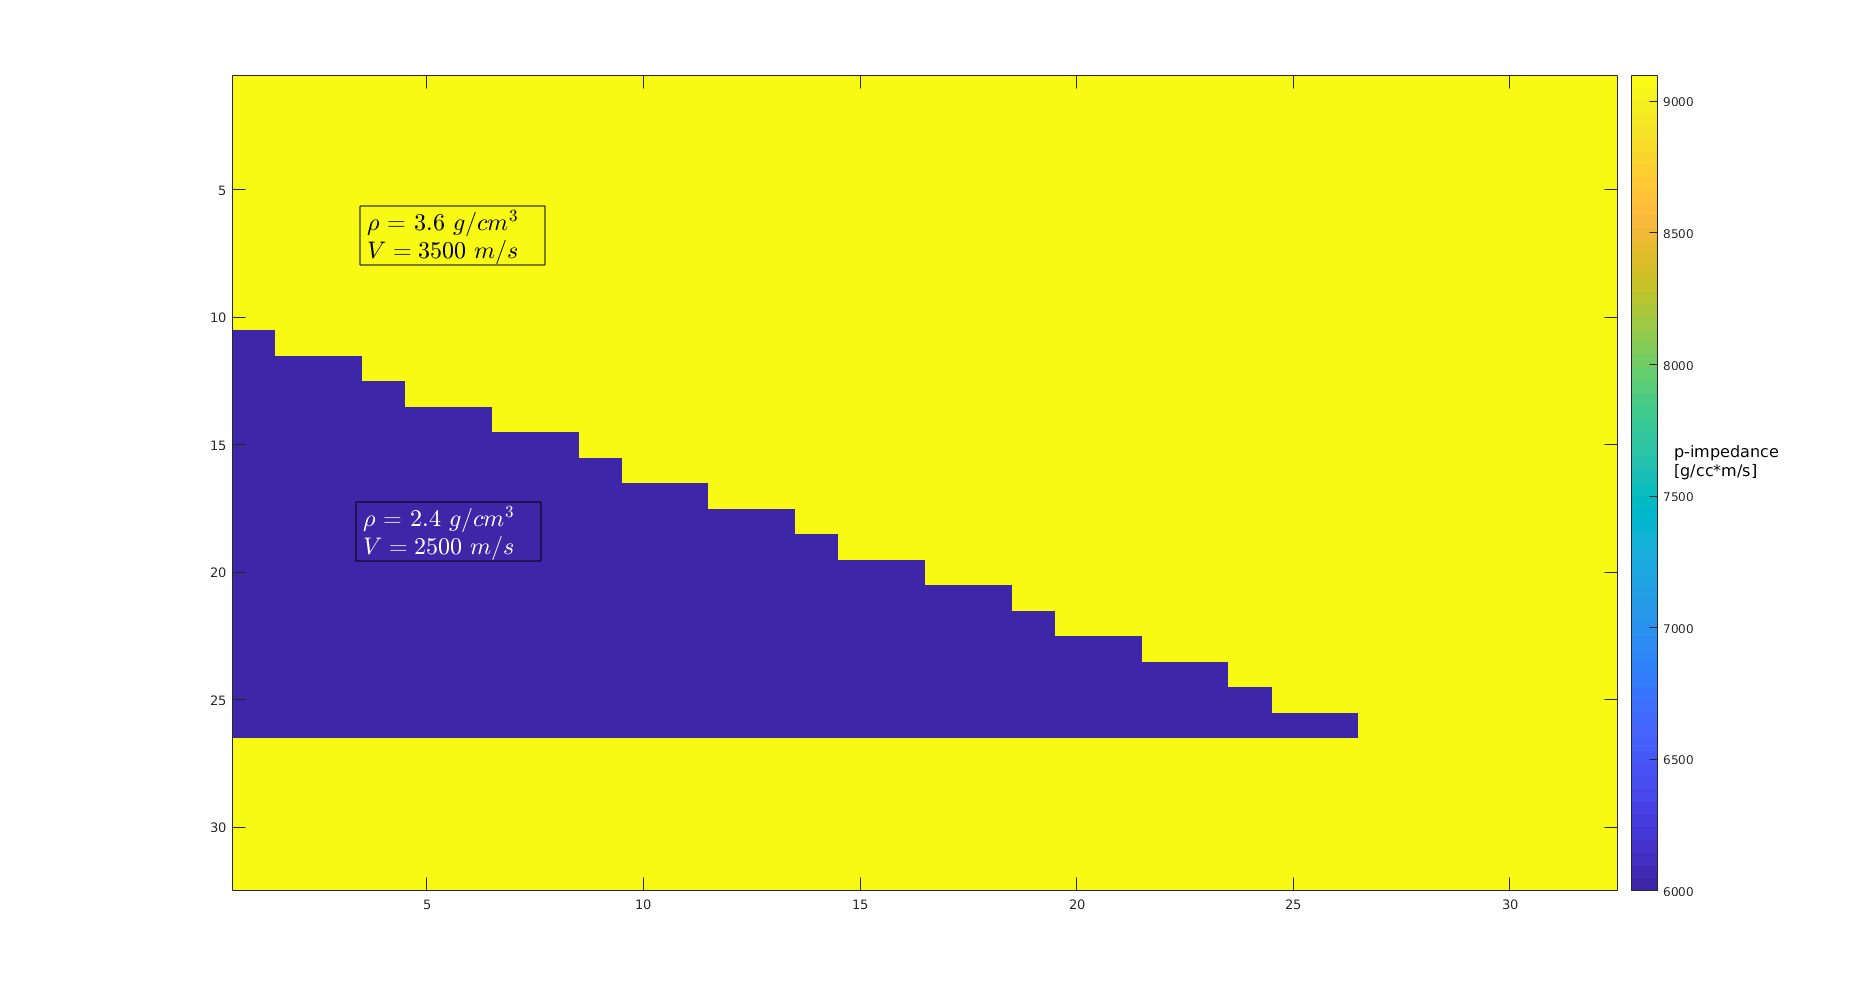
\includegraphics[width=3.0in]{Figs/Image_Paper}
\DeclareGraphicsExtensions.
\caption{Acoustic impedance blurred model.}
\label{fig_lithology}
\end{figure}
In a real scenario, the blurred acoustic impedance is the
result of an inversion method, that might be Maximum a Posteriori \cite{}, Sparse Spike \cite{} and Recursive Inversion \cite{}.
However, for experimental purpose, the acoustic impedance models were low-passed filtered
and the high frequencies were removed, this way we proceed the supervised training with high resolution and blurred images. The blurred image 
is illustrated in Fig. \ref{fig_blur}. To increase the number of examples in the training dataset we rotate the impedance models 
in integer multiples of right angle. This approach allows the model learning the maximum edge variabilities in wedges images.
\begin{figure}[!t]
\centering
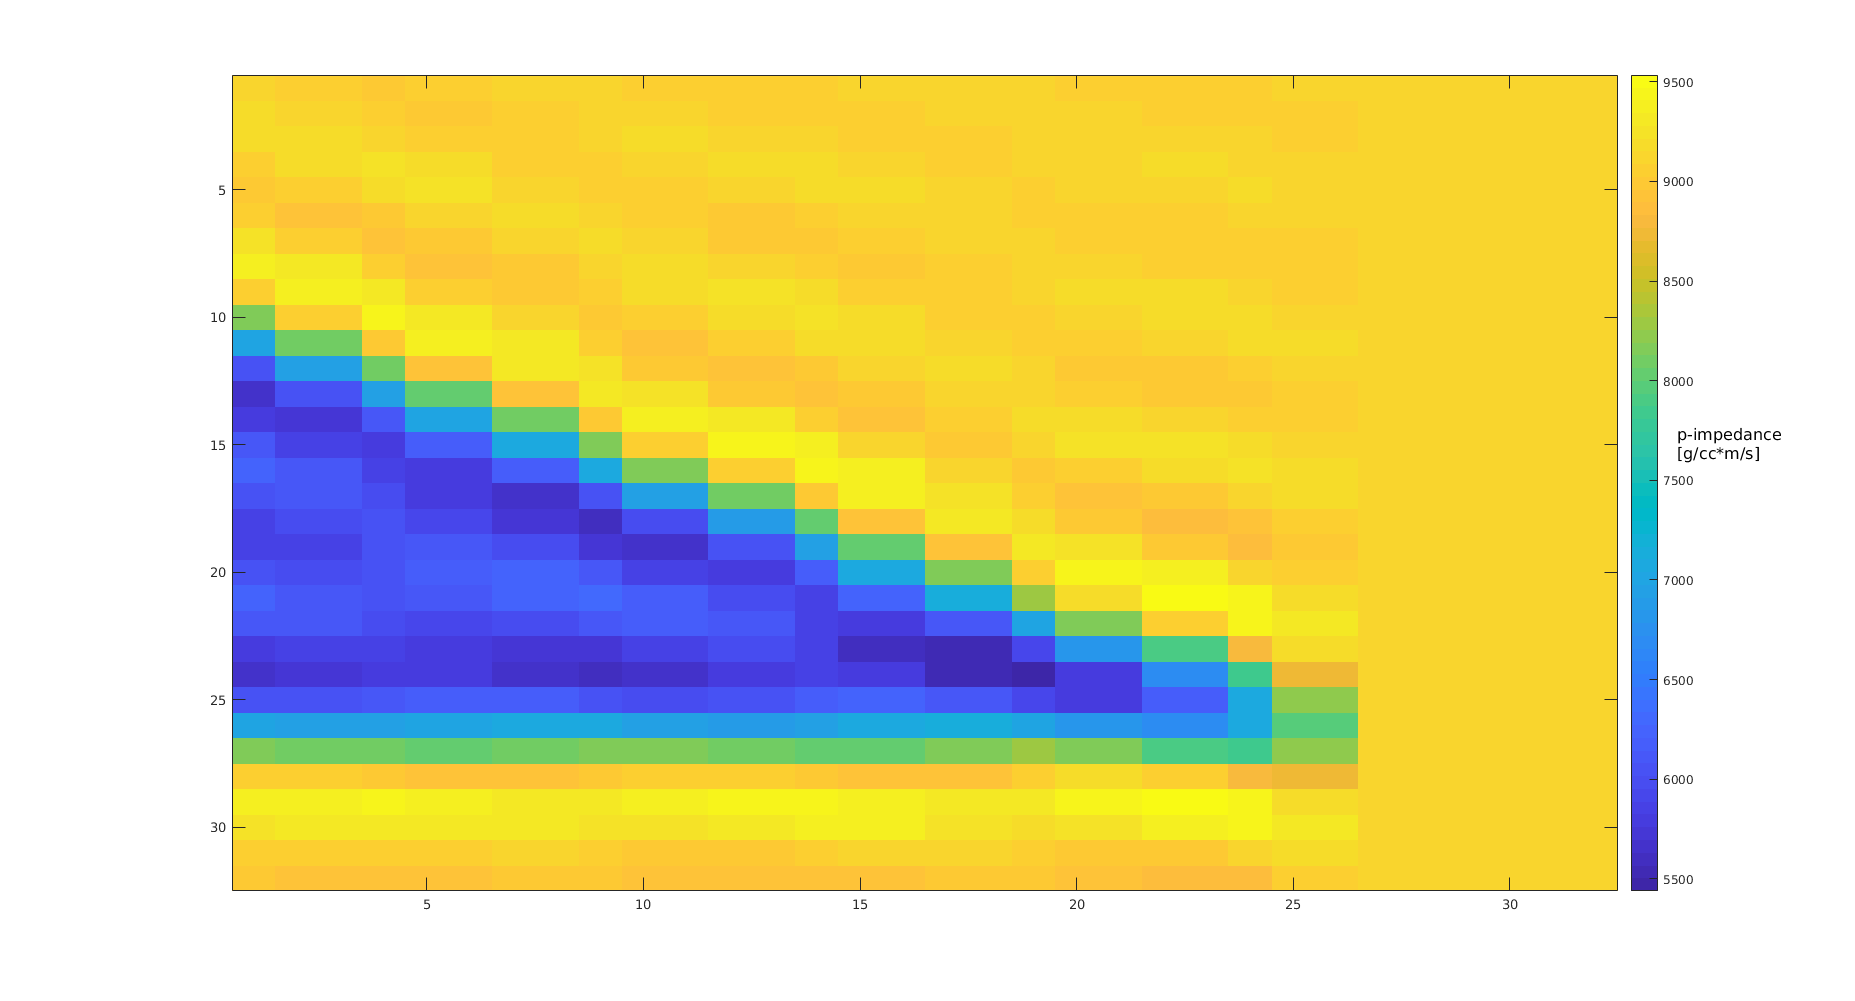
\includegraphics[width=3.0in]{Figs/Image_Paper_blurred}
\DeclareGraphicsExtensions.
\caption{Acoustic impedance blurred model.}
\label{fig_blur}
\end{figure}

\subsection{Convolutional Neural Network}
The work-flow of the proposed method consists of the following
steps:
\begin{itemize}
 \item Generate the synthetic impedance images;
 \item Blurr the images through a low-pass filter;
 \item Train the convolutional model with the pair of high and low resolution images;
 \item Test the model with different blurry images;
 \item Assess the result for the testing output.
\end{itemize}

The CNN is a well established method for
pattern recognition and image classification.
Thus, an important breakthrough when applying CNN to
deal with physical property images is developing a model
capable to solve regression tasks. The model presented in this paper
is able to solve two important problems related to deblurring physical properties
images: ($1$) learning the spacial patterns in the low resolution
training images and ($2$) predicting each pixel intensity value in the new
higher resolution image. To reach these two goals, the architecture of the
CNN contains convolutional layers combined with a regression output
layer.

The model proceeds a supervised learning through a dictionary containing pairs of low
and high resolution images. The optimization algorithm adjusts the 
network weights in every layer by minimizing the Mean Squared Error (MSE)
in each batch of images. Thus, after the training phase, the model is capable
to deblurr any other image not presented in training dataset. The output
image recovers the high frequencies and presents higher similarity
to the high resolution image than to the blurred image, according to stablished metric.
The model was adjusted to deblurr a wide variety
of wedges shapes and impedance values. Those wedges which the model was unable
to predict were added in the training set.

Three metrics assess the performance of the convolution networks: Fast Fourier Transform Index (FFTI),
the Rooted Mean Square Error (RMSE) and the frequencies magnitudes.
The FFTI is a similarity metric calculated based on the Fast Fourier Transform (FFT) of each image.
It is introduced by \cite{naranyana} and calculates as in Eq. \ref{eq:fourier}
\begin{equation}
 C = \frac{ (\sum_{i=1}^{N}{F_{1i}F_{2i}} - N \bar{F}_1\bar{F}_2 )^2 }{ (\sum_{i=1}^{N}{|F_{1i}|^2} - N{\bar{F}^2}_1)( \sum_{i=1}^{N}{|F_{2i}|^2} - N{\bar{F}^2}_2 )},
 \label{eq:fourier}
\end{equation}
where, for each frequency, an intensity value is calculated from the real and complex parts of fourier
transform. $F_{1i}$ represents the intensity value of $i$-th \textit{pixel} in the first image and $F_{2i}$
is the intensity value of $i$-th \textit{pixel} in the second image. $\bar{F}_1$ e $\bar{F}_2$ are the mean
frequencies in each image. The closer FFTI is to $1$, the higher the similarity between the images.
The frequencies spectrum is additionally useful to present the graphic of frequency magnitudes in the images.
The frequency magnitude graphic allows distinguishing what high frequencies were added to the acoustic impedance
after the low resolution image is passed through the trained CNN. 
Additionally, the Root Mean Squared Error (RMSE) in Eq. \ref{eq:mse} is calculated in order to measure
the global error in each pair of deblurred and high resolution images.

\begin{equation}
 RMSE = \sqrt{\frac{ (\sum_{i=1}^{N}{(x_i -y_i)^2 } }{N}},
 \label{eq:mse}
\end{equation}

The model architecture consists in two convolution layers, each one followed by one
pooling layer and a regularization layer. The second regularization layer is followed
by a fully connected layer, which maps the convolution layer's output to $1024$ neurons.
The output model comprises a regression layer to predict the intensity value of each pixel.

\section{Experiments}
%This section describes the experiments and results obtained with the proposed method.
%We compare the results with the state-of-the-art deblurring algorithms in four different scenarios.
To build the training dataset we generated $500$ random wedge 
images. Each image was rotated in four angles integer multiple of $90$
degrees, then comprising a total of $2000$ images. 
By rotating the images, we aimed to present to the network the 
lithologies in different positions and expected the network
to identify a general sort of wedges in angles different from integer
multiples of $90$ degrees. The rotated images were blurred by applying a low-pass filter with
cut frequency $4Hz$ and the pairs of blurred and not-blurred images were used to
adjust the model weights. The same approach was applied to generate different
scenarios for test cases. Some scenarios do probably not
address a geological meaning, however, we have with them evaluated the capability of the model
in deblurring and predicting a wide sort of acoustic impedance images.

% In the first scenario we trained and tested the network with images of acoustic impedance normalized to $0$ and $1$.
% This scenario evaluated the model capability to deblurr lithology with similar acoustic impedance
% values as in the training dataset, but with different shapes. 
% In the second scenario, we  inverted the lithology impedance values in the test images to evaluate the ability of the 
% network to predict the correct impedance value, despite the position of the a pixel on the image. 
% The fourth scenario tested images with different acoustic impedance values and
% different wedge shapes and rotations, in comparison to the images used in the training phase.
% In this case we tested the model capability to deblurr different wedge shapes, located in
% different positions, and to extrapolate the acoustic impedance values.

\subsection{Implementation Details}
The model was implemented using the Deep Learning toolbox
delivered in MATLAB R2017A. For training the network, we used a mini-batch with size of $32$ training examples.
The network weights are randomly initialized and the Stochastic Gradient Descendant with
Momentum (SGDM) \cite{Ning}. We adopted an exponentially decreasing learning rate (initially
set to $0.005$), decreasing every iteration in a total of $100$ iterations.
It should be noted that, once the wedge shapes are randomly generated, every image is different
and each one was introduced only once to the network, this way avoiding over-fitting.

\subsection{Integer Angles Rotated Wedges}

In the first scenario, we used acoustic impedance images
with the same rotation and impedance values as the images in the
training dataset. The wedges in the testing set differ from
the the ones in the training set only by their shapes.
\begin{figure}[!t]
\centering
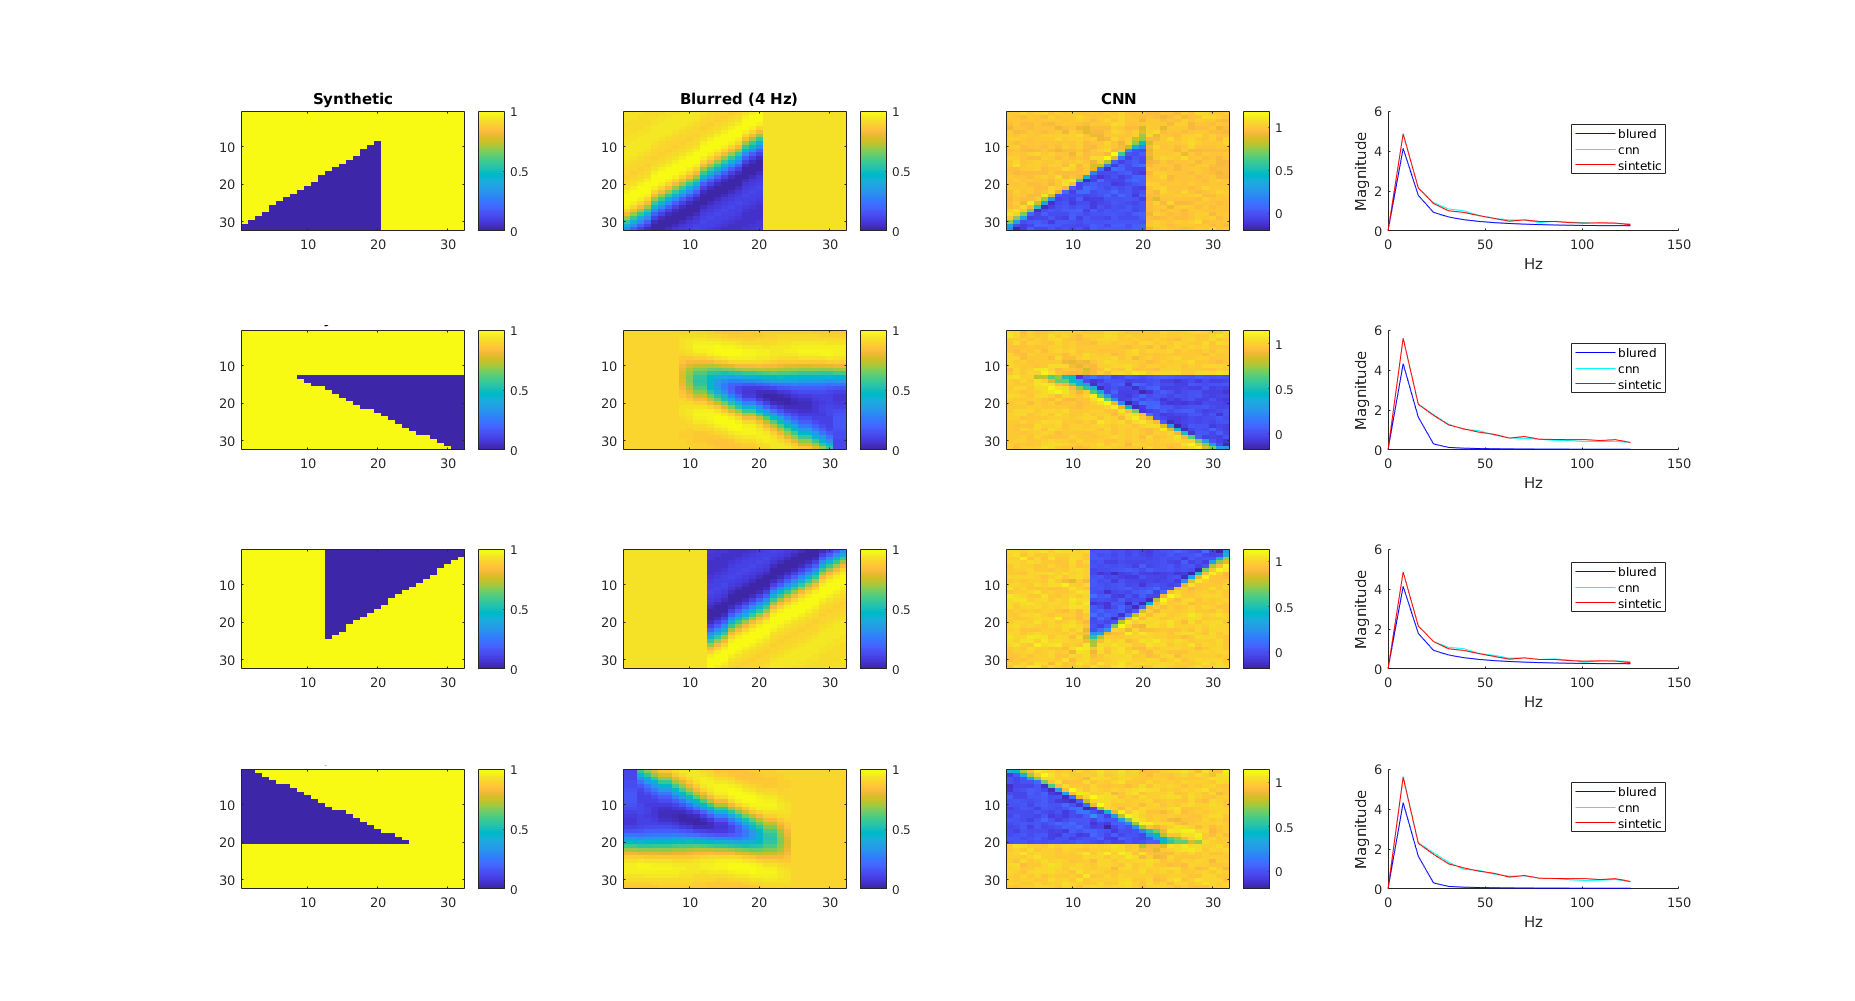
\includegraphics[width=3.0in]{Figs/Caso1}
\DeclareGraphicsExtensions.
\caption{Acoustic impedance blurred model.}
\label{fig_scenario1}
\end{figure}
Fig. \ref{fig_scenario1} presents the result obtained with the initial model applied to the
test images. The first column shows the high resolution images followed
by the blurred images, the third column shows the result of the convolutional deblurring network
and the fourth column shows the graph of frequency magnitudes of each image
(synthetic, blurred and CNN).
%Explicar os resultados dos indices

In the second scenario, we inverted the impedance values of the lithology structures.
This way we verified that the prediction of the pixel value is disconnected to the lithology shape.
Fig. \ref{fig_scenario6} shows the results obtained in this scenario.
\begin{figure}[!t]
\centering
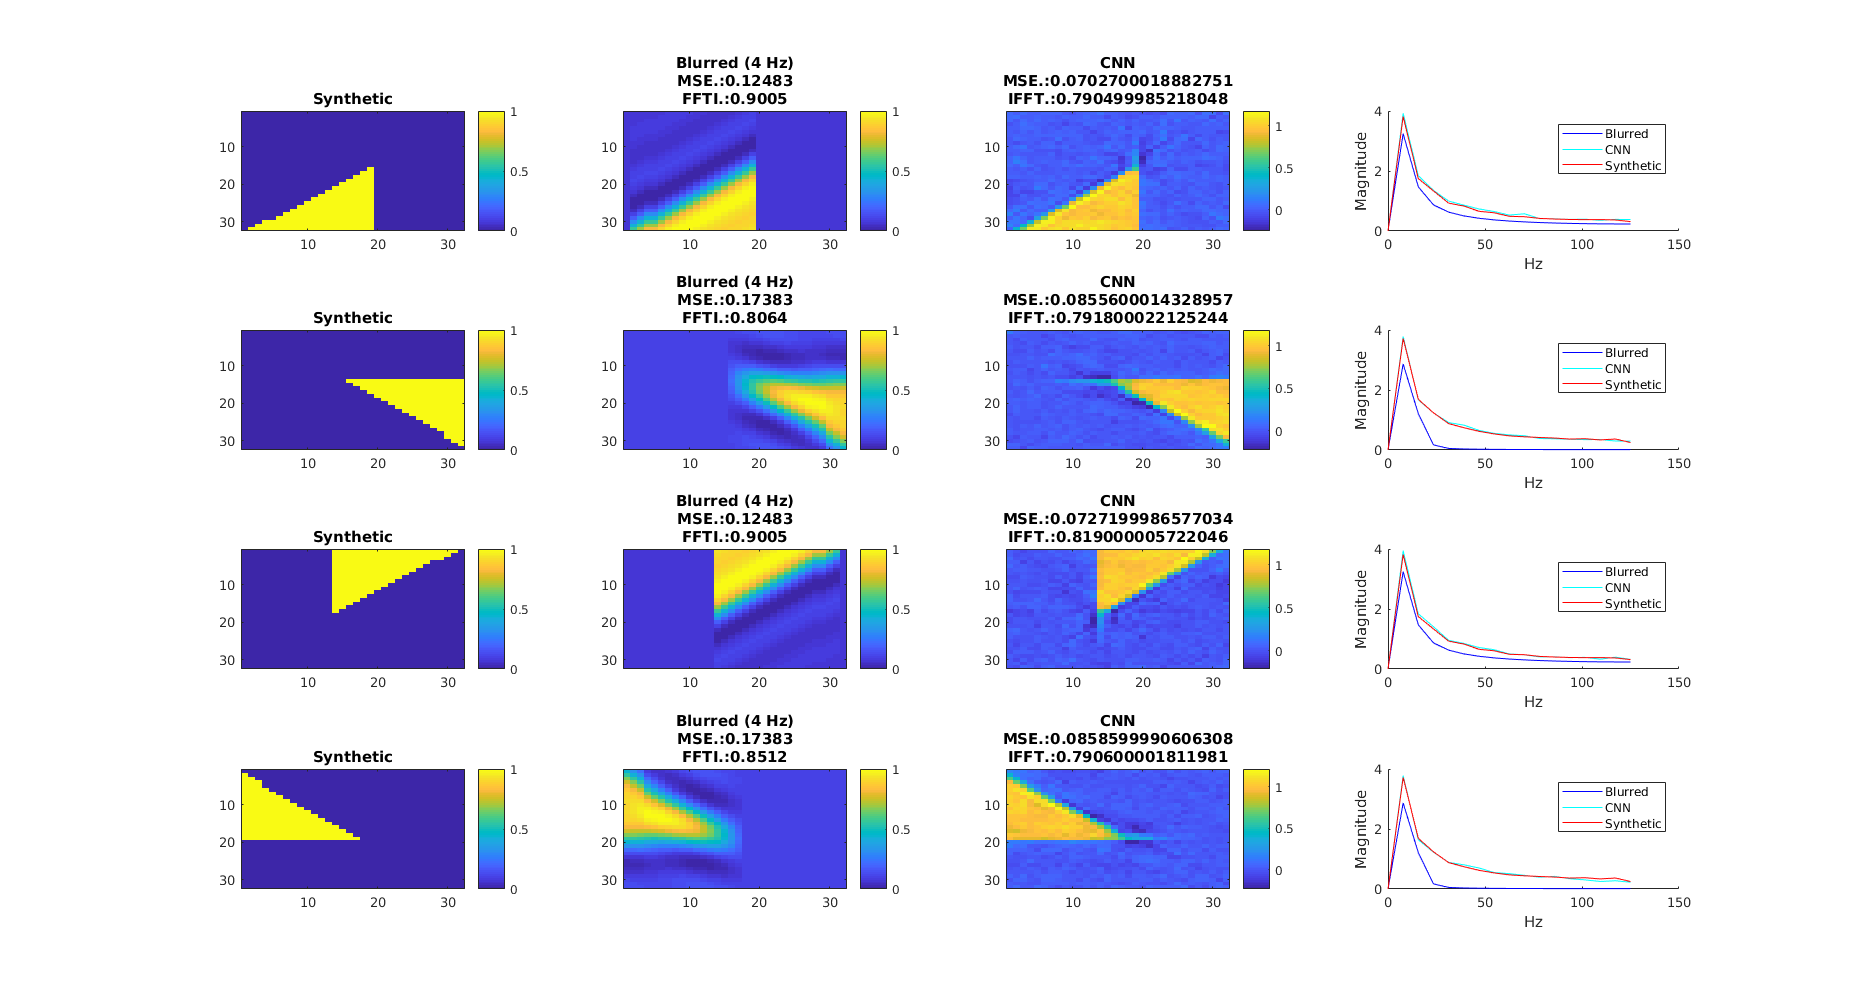
\includegraphics[width=3.0in]{Figs/Caso6}
\DeclareGraphicsExtensions.
\caption{Acoustic impedance blurred with inverted property values.}
\label{fig_scenario6}
\end{figure}

In the third scenario, we arbitrarily changed the normalized impedance to values
of higher impedance out of the wedge (with value of $0.7$) and lower impedance (with value of $0.3$)
into the wedge. These values are out the range learned by the model during the training phase.
Doing this, we tested the model generalization capacity to reach the learned pixel intensity values.
We observed that, once the model is trained with pixel valued to $0$ and $1$, the network poorly
extrapolated and a new training dataset was generated containing wedges with the new pixel values.
The Fig. \ref{fig_scenario2} shows the result for the network trained with the extended dataset.
\begin{figure}[!t]
\centering
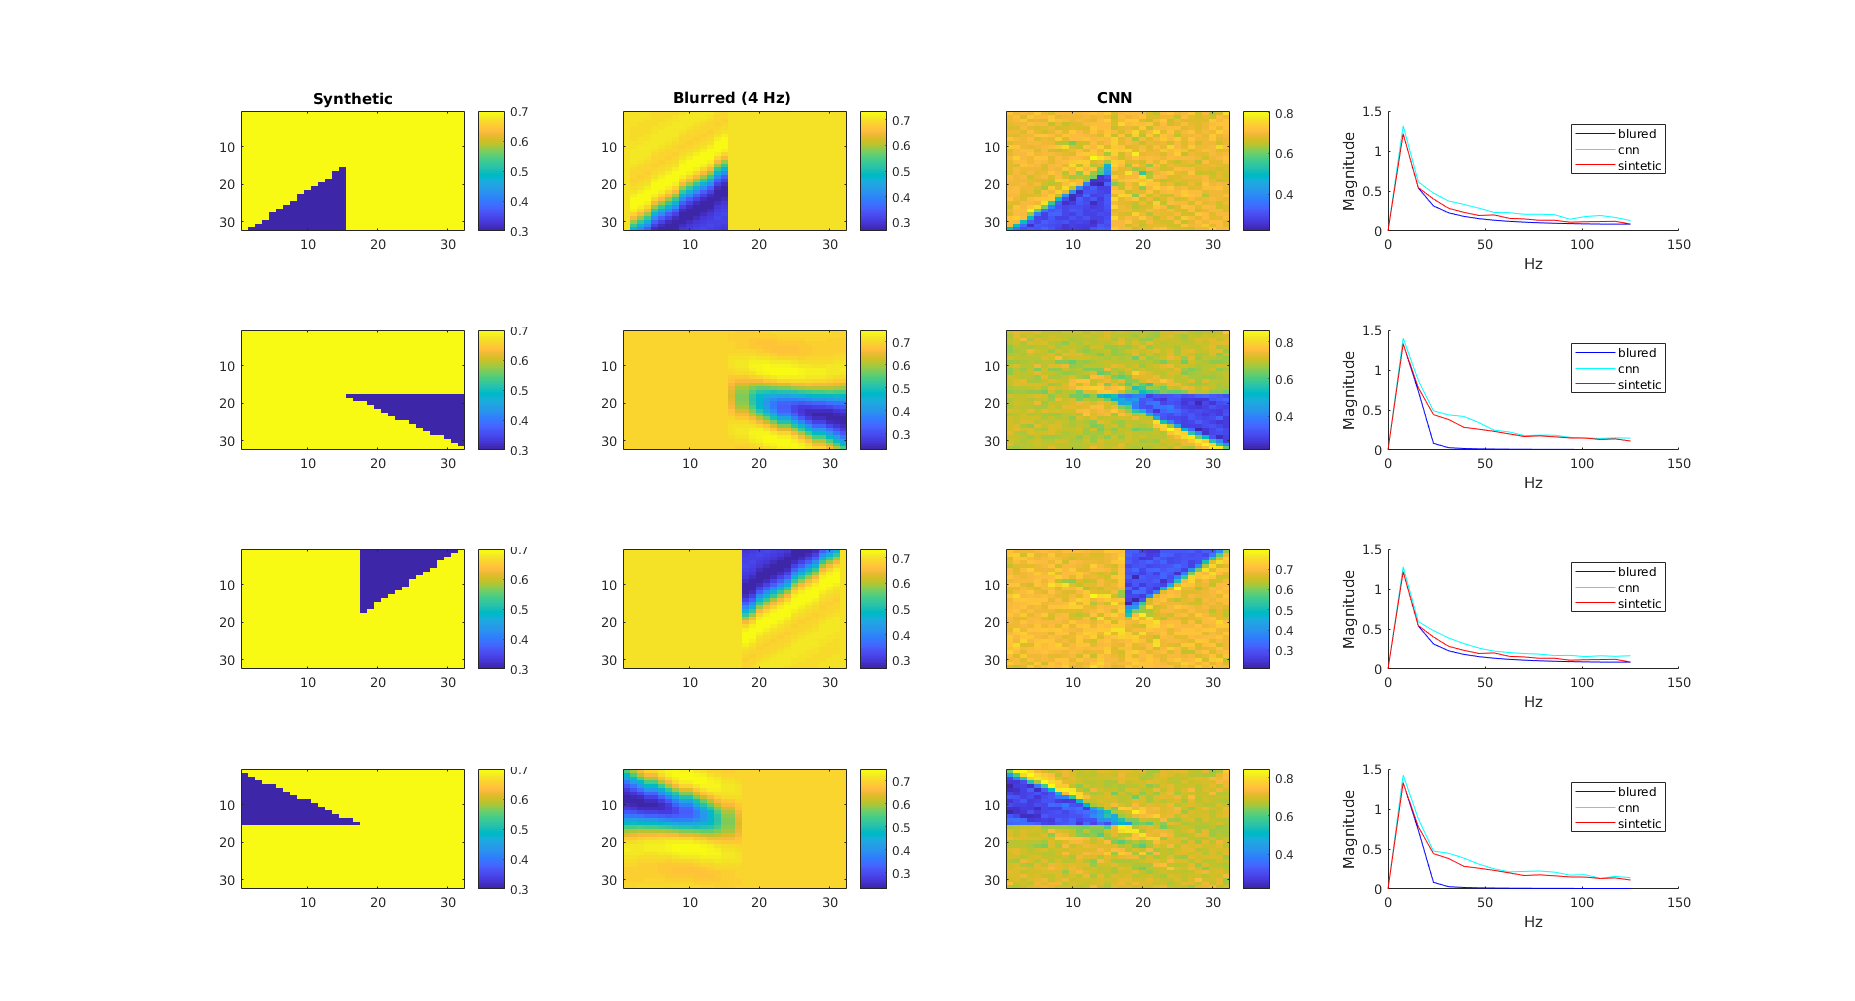
\includegraphics[width=3.0in]{Figs/Caso2}
\DeclareGraphicsExtensions.
\caption{Acoustic impedance normalized to arbitrary values.}
\label{fig_scenario2}
\end{figure}

%Explicar os resultados dos indices para este cenário

A new scenario was simulated, in which the  synthetic images were blurred with different
cut frequencies. Each one of the four test images was blurred with a cut frequency
randomly chosen between $3$ and $20$ Hz. This is particularly interesting, because
in a scenario with real data, physical aspects as signal attenuation may lead to
different blurring profiles in post-inversion images.
Fig. \ref{fig_scenario5} shows the results for this scenarios.
\begin{figure}[!t]
\centering
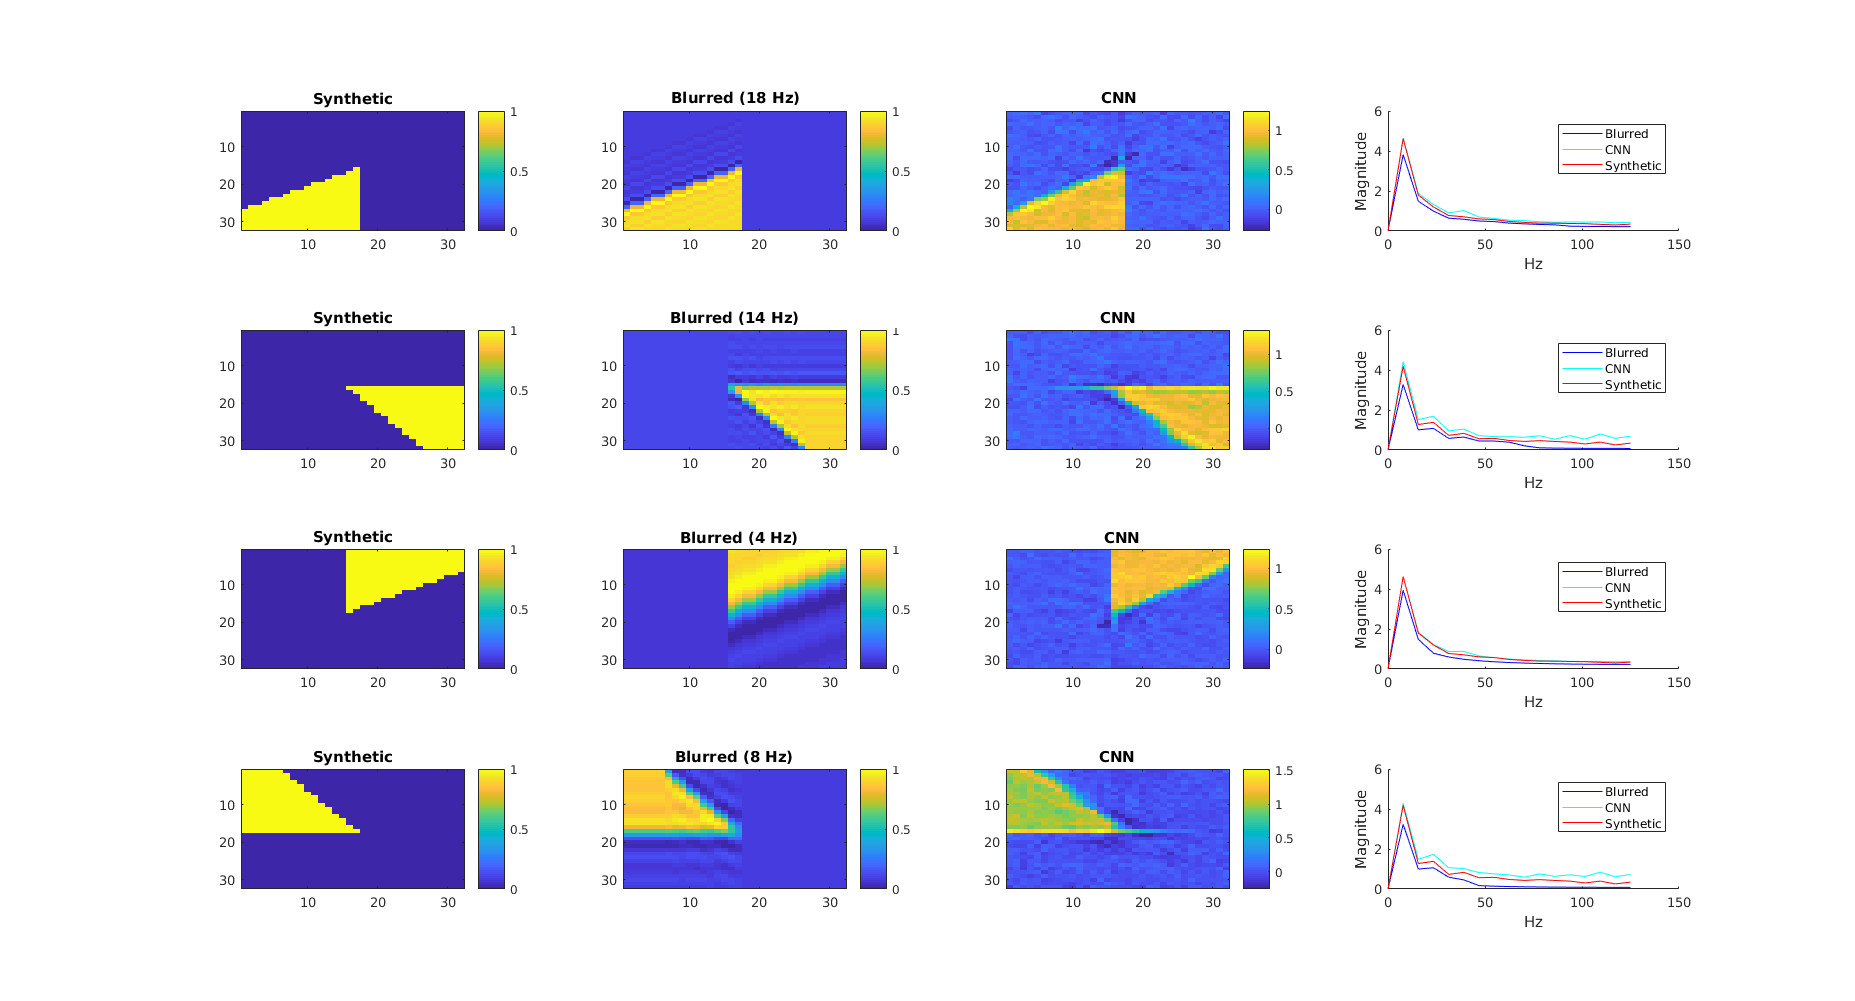
\includegraphics[width=3.0in]{Figs/Caso5}
\DeclareGraphicsExtensions.
\caption{Acoustic impedance blurred with different frequencies.}
\label{fig_scenario5}
\end{figure}

\subsection{Randomly Rotated Wedges}
Randomly rotated wedge is related to a lithology positioned in a random angle.
In this case, we evaluated the CNN capability to deblurr the lithologies with shape and position absent
in the training dataset. As in the previews tests, the model was trained with lithologies rotated
in integer multiple of the right angle and the model was expected to identify the edges and contours of the wedges,
and recover the correct values of impedance.
Fig. \ref{fig_scenario4} shows the test case in which the acoustic impedance was generated with values $0$ and $1$.
As the network was trained with wedges with the same value, the network was able to predict
the pixel intensity value.
\begin{figure}[!t]
\centering
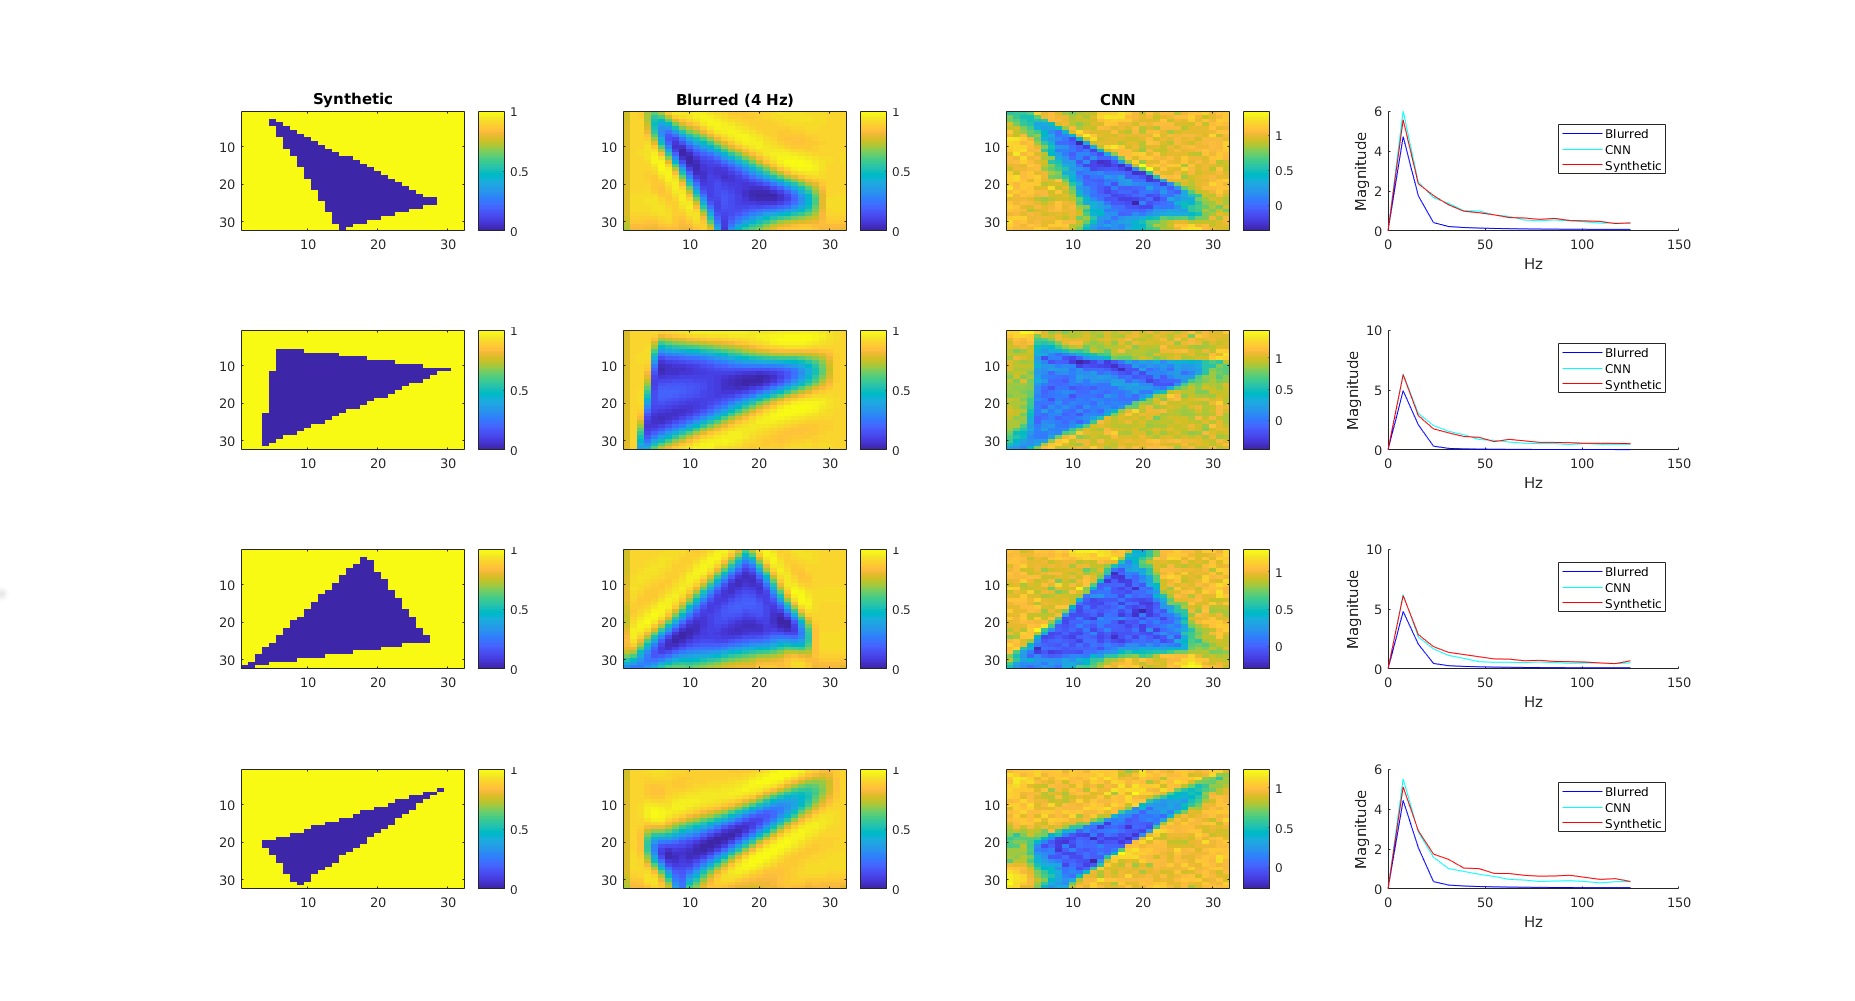
\includegraphics[width=3.0in]{Figs/Caso4}
\DeclareGraphicsExtensions.
\caption{Acoustic impedance blurred model.}
\label{fig_scenario4}
\end{figure}

Fig. \ref{fig_scenario3} shows the test case in which the wedges were positioned in random angles and the acoustic impedance
was normalized to values equal to $0.3$ and $0.7$. These values were absent in the training dataset and it
is notable a wider spread of values in both lithologies outputted by the network.
\begin{figure}[!t]
\centering
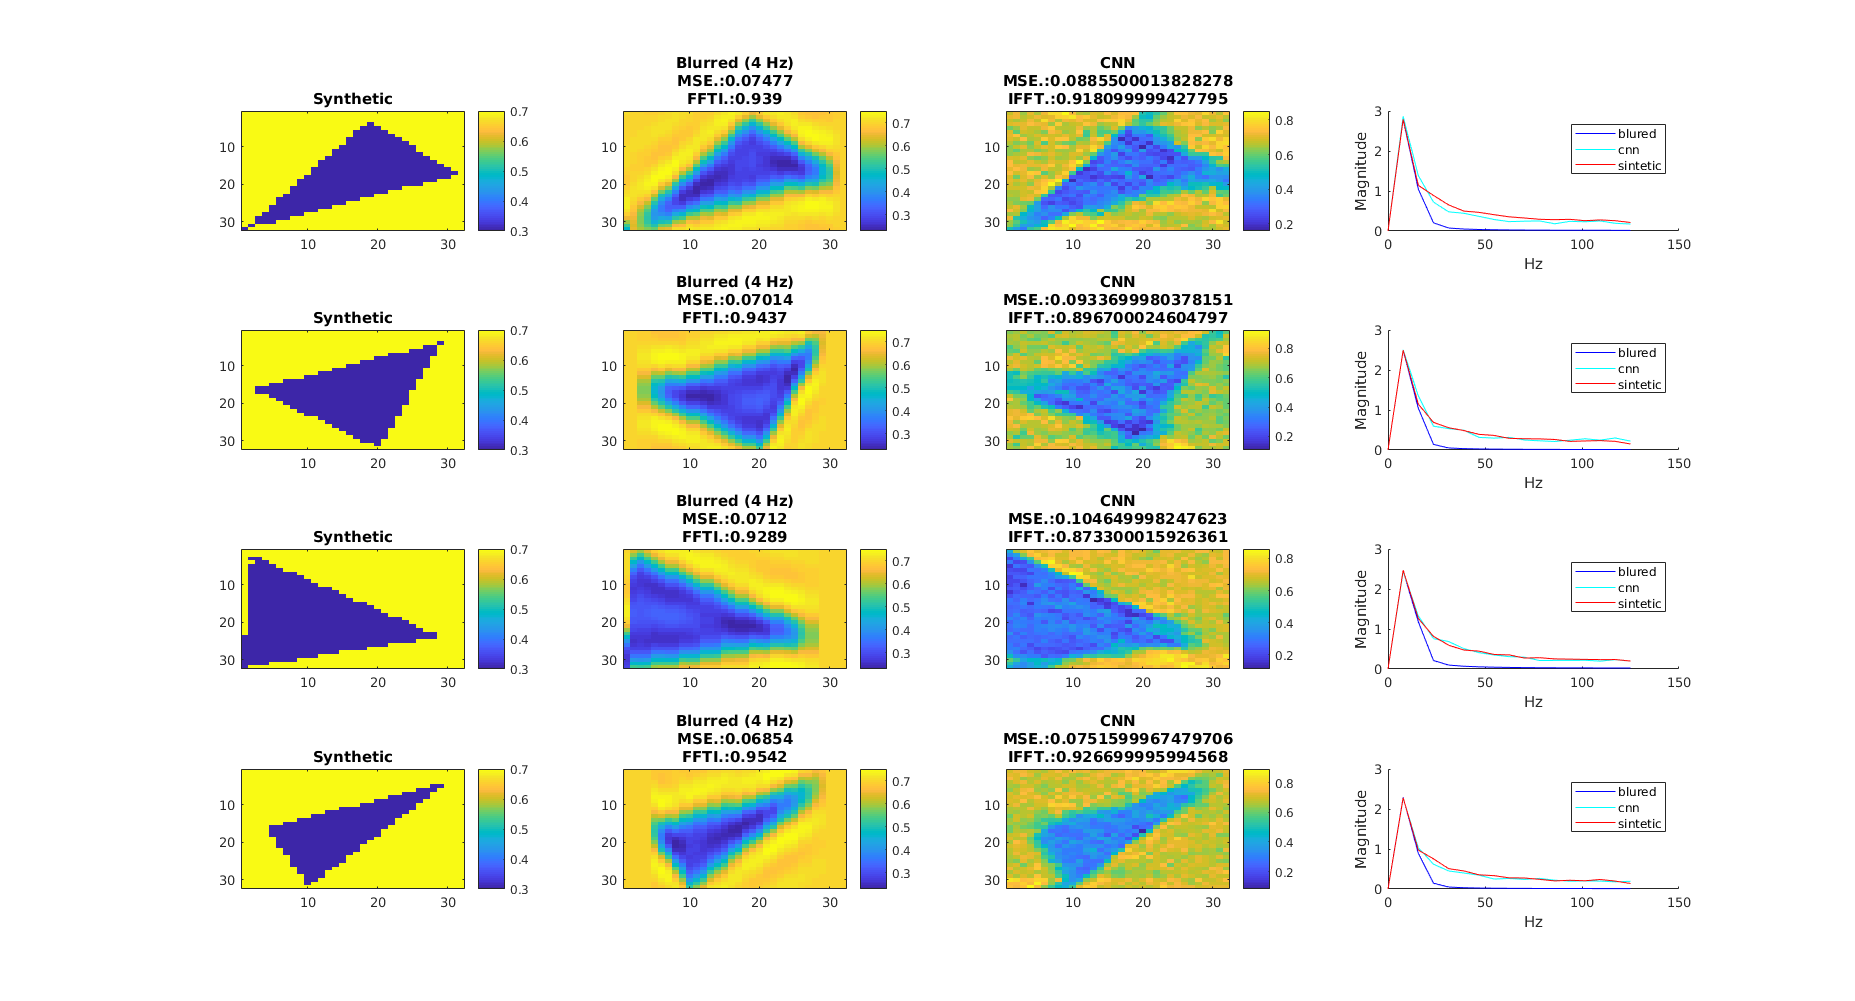
\includegraphics[width=3.0in]{Figs/Caso3}
\DeclareGraphicsExtensions.
\caption{Acoustic impedance blurred model.}
\label{fig_scenario3}
\end{figure}
%
% Reminder: the "draftcls" or "draftclsnofoot", not "draft", class
% option should be used if it is desired that the figures are to be
% displayed while in draft mode.
%
%\begin{figure}[!t]
%\centering
%\includegraphics[width=2.5in]{myfigure}
% where an .eps filename suffix will be assumed under latex, 
% and a .pdf suffix will be assumed for pdflatex; or what has been declared
% via \DeclareGraphicsExtensions.
%\caption{Simulation results for the network.}
%\label{fig_sim}
%\end{figure}

% Note that the IEEE typically puts floats only at the top, even when this
% results in a large percentage of a column being occupied by floats.


% An example of a double column floating figure using two subfigures.
% (The subfig.sty package must be loaded for this to work.)
% The subfigure \label commands are set within each subfloat command,
% and the \label for the overall figure must come after \caption.
% \hfil is used as a separator to get equal spacing.
% Watch out that the combined width of all the subfigures on a 
% line do not exceed the text width or a line break will occur.
%
%\begin{figure*}[!t]
%\centering
%\subfloat[Case I]{\includegraphics[width=2.5in]{box}%
%\label{fig_first_case}}
%\hfil
%\subfloat[Case II]{\includegraphics[width=2.5in]{box}%
%\label{fig_second_case}}
%\caption{Simulation results for the network.}
%\label{fig_sim}
%\end{figure*}
%
% Note that often IEEE papers with subfigures do not employ subfigure
% captions (using the optional argument to \subfloat[]), but instead will
% reference/describe all of them (a), (b), etc., within the main caption.
% Be aware that for subfig.sty to generate the (a), (b), etc., subfigure
% labels, the optional argument to \subfloat must be present. If a
% subcaption is not desired, just leave its contents blank,
% e.g., \subfloat[].


% An example of a floating table. Note that, for IEEE style tables, the
% \caption command should come BEFORE the table and, given that table
% captions serve much like titles, are usually capitalized except for words
% such as a, an, and, as, at, but, by, for, in, nor, of, on, or, the, to
% and up, which are usually not capitalized unless they are the first or
% last word of the caption. Table text will default to \footnotesize as
% the IEEE normally uses this smaller font for tables.
% The \label must come after \caption as always.
%
%\begin{table}[!t]
%% increase table row spacing, adjust to taste
%\renewcommand{\arraystretch}{1.3}
% if using array.sty, it might be a good idea to tweak the value of
% \extrarowheight as needed to properly center the text within the cells
%\caption{An Example of a Table}
%\label{table_example}
%\centering
%% Some packages, such as MDW tools, offer better commands for making tables
%% than the plain LaTeX2e tabular which is used here.
%\begin{tabular}{|c||c|}
%\hline
%One & Two\\
%\hline
%Three & Four\\
%\hline
%\end{tabular}
%\end{table}


% Note that the IEEE does not put floats in the very first column
% - or typically anywhere on the first page for that matter. Also,
% in-text middle ("here") positioning is typically not used, but it
% is allowed and encouraged for Computer Society conferences (but
% not Computer Society journals). Most IEEE journals/conferences use
% top floats exclusively. 
% Note that, LaTeX2e, unlike IEEE journals/conferences, places
% footnotes above bottom floats. This can be corrected via the
% \fnbelowfloat command of the stfloats package.




\section{Conclusion}
The conclusion goes here.



% use section* for acknowledgment
\ifCLASSOPTIONcompsoc
  % The Computer Society usually uses the plural form
  \section*{Acknowledgments}
\else
  % regular IEEE prefers the singular form
  \section*{Acknowledgment}
\fi


The authors would like to thank...





% trigger a \newpage just before the given reference
% number - used to balance the columns on the last page
% adjust value as needed - may need to be readjusted if
% the document is modified later
%\IEEEtriggeratref{8}
% The "triggered" command can be changed if desired:
%\IEEEtriggercmd{\enlargethispage{-5in}}

% references section

% can use a bibliography generated by BibTeX as a .bbl file
% BibTeX documentation can be easily obtained at:
% http://mirror.ctan.org/biblio/bibtex/contrib/doc/
% The IEEEtran BibTeX style support page is at:
% http://www.michaelshell.org/tex/ieeetran/bibtex/
%\bibliographystyle{IEEEtran}
% argument is your BibTeX string definitions and bibliography database(s)
%\bibliography{IEEEabrv,../bib/paper}
%
% <OR> manually copy in the resultant .bbl file
% set second argument of \begin to the number of references
% (used to reserve space for the reference number labels box)
\begin{thebibliography}{1}

\bibitem{IEEEhowto:kopka} 	H.~Kopka and P.~W. Daly, \emph{A Guide to \LaTeX}, 3rd~ed.\hskip 1em plus 0.5em minus 0.4em\relax Harlow, England: Addison-Wesley, 1999.
\bibitem{xiaoiu}  		Xi Xiaoyu, Ling Yun, Sun Desheng, Guo Xiangyu, and Wang Huifeng, ``Studying the effect of expanding low or high frequency on post-stack seismic inversion,'' in SEG Technical Program Expanded Abstracts 2012. September 2012, 1-5.
\bibitem{Buduma15}  		Buduma, N., `` Fundamentals of Deep Learning,'' Academic Press, 2015, in O'Reilly Media.
\bibitem{qian} 			Qian Feng, Yin Miao, Su Ming-Jun, Wang Yaojun, Hu Guangmin, ``Seismic facies recognition based on prestack data using deep convolutional autoencoder,''.
\bibitem{Liu} 			Liu Lihui, Lu Rong, Li Jianhai, Yang Wenkui, ``Seismic Lithofacies Computation Method Based on Deep Learning,'' p. 649-652.
\bibitem{Chrysos} 		G. G. Chrysos, S. Zafeiriou, "Deep Face Deblurring," 2017 IEEE Conference on Computer Vision and Pattern Recognition Workshops (CVPRW), Honolulu, HI, 2017, pp. 2015-2024.
\bibitem{Latimer} 		Rebecca Buxton Latimer, Rick Davidson, Paul van Riel, ``An interpreter's guide to understanding and working with seismic-derived acoustic impedance data,'',2017, pp. 242-256, v. 19, num. 3, in The Leading Edge.
\bibitem{buiting} 		JJM. Buiting, M. Bacon,``Using geophysical, geological, and petrophysical data to characterize reservoirs in the North Sea.'', in 5th Conference on Petroleum Geology of NW Europe, London. CD-ROM.
\bibitem{riel} 			Paul van Riel,  ``The past, present and future of quantitative reservoir characterization.'', in The Leading Edge, 19, p. 878–881.
\bibitem{sergio}		Sergio Sacani Sancevero, Armando Zaupa Remacre, Rodrigo de Souza Portugal, ``O papel da inversão para a impedância no processo de caracterização sísmica de reservatórios'',in Revista Brasileira de Geofísica, 2006, p. 495-512, v. 24.
\bibitem{Russakovsky}		O. Russakovsky, J. Deng, H. Su, J. Krause, S. Satheesh, S. Ma, Z. Huang, A. Karpathy, A. Khosla, M. Bernstein, ``Imagenet large scale visual recognition challenge,'' in ternational Journal of Computer Vision (IJCV), p. 211–252, 2015.
\bibitem{Girshick}		R. Girshick, ``Fast r-cnn,'' In IEEE Proceedings of International Conference on Computer Vision (ICCV), pages 1440–1448, 2015.
\bibitem{Bell} 			S. Bell, C. L. Zitnick, K. Bala, and R. Girshick, ``Inside-outside net: Detecting objects in context with skip pooling and recurrent neural networks,'' in arXiv preprint arXiv:1512.04143, 2015.s
\bibitem{Nam}			H. Nam and B. Han, ``Learning multi-domain convolutional neural networks for visual tracking,'' In IEEE Proceedings of International Conference on Computer Vision and Pattern Recognition (CVPR). IEEE, 2016.
\bibitem{He}			K. He, X. Zhang, S. Ren, and J. Sun, ``Deep residual learning for image recognition,'' In IEEE Proceedings of International Conference on Computer Vision and Pattern Recognition (CVPR). IEEE, 2016.
\bibitem{Levin}			A. Levin, Y. Weiss, F. Durand, and W. T. Freeman. ``Understanding and evaluating blind deconvolution algorithms.'' In IEEE Proceedings of International Conference on Computer Vision and Pattern Recognition (CVPR), p. 1964–1971.
\bibitem{Levin2011}		A. Levin, Y. Weiss, F. Durand, and W. T. Freeman. ``Efficient marginal likelihood optimization in blind deconvolution.'' In CVPR, 2011.
\bibitem{Krizhevsky}		A. Krizhevsky, I. Sutskever, G. E. Hinton, ``Imagenet classification with deep convolutional neural networks: Advances in neural information processing systems,'' 2012, p. 1097–1105.
\bibitem{S_Ji}			S. Ji,W. Xu, M. Yang, K. Yu, 2013, ``3d convolutional neural networks for human action recognition,'' in IEEE transactions on pattern analysis and machine intelligence, n. 35, p. 221–231.
\bibitem{AbdelHamid}		O. Abdel-Hamid, A.-r. Mohamed, H. Jiang, L. Deng, G. Penn, D. Yu, 2014, ``Convolutional neural networks for speech recognition,'' in IEEE/ACM Transactions on audio, speech, and language processing, n. 22, p. 1533–1545.
\bibitem{Farfade}		S. S. Farfade, M. J. Saberian, L.-J. Li, 2015, ``Multi-view face detection using deep convolutional neural networks,'' in Proceedings of the 5th ACM on International Conference on Multimedia Retrieval, ACM, p. 643–650.
\bibitem{Harvey} 		P. J. Harvey, D. J. MacDONALD, ``Seismic modelling of porosity within the jurassic aged carbonate bank, offshore Nova Scotia,'' in  Canadian Journal of Exploration Geophysics, n. 26, p. 54–71.
\bibitem{naranyana}		S. Narayana, P. K. Thirivikraman, ``Image similarity using fourier transform,'' in International Journal of Computer Engeneering and Technology, 2015, n. 6, p. 29–37.
\bibitem{Ning}			N. Qian, ``On the momentum term in gradient descent learning algorithms,'' in Neural Networks, v. 12, i. 1, 1999, p. 145-151.
\bibitem{bishop}		T.E. Bishop, S.D. Babacan, Amizic, T. Chan, R. Molina, A. Katsaggelos, ``Blind image deconvolution: problem formulation and existing approaches.'' in. Blindimage deconvolution: theory and applications,  CRC press (2007).
\bibitem{babacan}		S. D. Babacan, R. Molina, M. N. Do, and A. K. Katsaggelos, ``Bayesian blind deconvolution with general sparse image priors.'' In. Proceedings of European Conference on Computer Vision (ECCV), p. 341–355, 2012.
\bibitem{Hacohen2013}		Y. Hacohen, E. Shechtman, and D. Lischinski, ``Deblurring by example using dense correspondence.'' In IEEE Proceedings of International Conference on Computer Vision (ICCV), p. 2384–2391, 2013.
\bibitem{Pan2014}		J. Pan, Z. Hu, Z. Su, M. H. Yang., ``Deblurring face images with exemplars.'' In Proceedings of European Conference on Computer Vision (ECCV), p. 47–62. Springer, 2014.
\bibitem{Lai2016}		W.S. Lai, J. B. Huang, Z. Hu, N. Ahuja, M. H. Yang.``A comparative study for single image blind deblurring.'' In IEEE Proceedings of International Conference on Computer Vision and Pattern Recognition (CVPR). IEEE, 2016.
\bibitem{Chakrabarti2016}	A. Chakrabarti. ``A neural approach to blind motion deblurring.'' In Proceedings of European Conference on Computer Vision (ECCV), p. 221–235. Springer, 2016.
\bibitem{Hradis2015}		M. Hradiš, J. Kotera, P. Zemcı́k, F. Šroubek. ``Convolutional neural networks for direct text deblurring.'' In Proceedings of British Machine Vision Conference (BMVC), 2015.
\bibitem{Sun2015}		J. Sun, W. Cao, Z. Xu, J. Ponce. ``Learning a convolutional neural network for non-uniform motion blur removal.'' In IEEE Proceedings of International Conference on Computer Vision and Pattern Recognition (CVPR), p. 769–777, 2015.
\bibitem{Krishnan2015}		D. Krishnan, T. Tay, R. Fergus. ``Blind deconvolution using anormalized sparsity measure.'' In CVPR, 2011.
\bibitem{Zhang2011}		H. Zhang, J. Yang, Y. Zhang, N. M. Nasrabadi, T. S. Huang. ``Close the loop: Joint blind image restoration and recognition with sparse representation prior.'' In ICCV, 2011. 
\bibitem{sroubek2012}		F. Šroubek and P. Milanfar. ``Robust multichannel blind deconvolution via fast alternating minimization.'' in IEEE Trans. on Image Processing, p. 1687–1700, 2012.
\bibitem{Zhu2012}		X. Zhu, F. Šroubek, P. Milanfar. ``Deconvolving PSFs for a better motion deblurring using multiple images.'' In ECCV, 2012.
\bibitem{Figueiredo2012}	L. P. Figueiredo, M. Santos, M. Roisenberg, G. Neto, W. Figueiredo, ``Bayesian framework to wavelet estimation and linearized acoustic inversion,'' In Geoscience and Remote Sensing Letters, 2012, p. 1–5.
\bibitem{Buland2003}		A. Buland,  H. Omre, ``Bayesian linearized avo inversion,'' In Geophysics, 2003, p. 185–198.

\end{thebibliography}

%0 Journal Article
%A Rebecca Buxton Latimer
%A Rick Davidson
%A Paul van Riel
%T An interpreter's guide to understanding and working with seismic-derived acoustic impedance data
%D 2000
%J The Leading Edge
%P 242-256
%V 19
%N 3
%R 10.1190/1.1438580
%U http://library.seg.org/doi/abs/10.1190/1.1438580
%K 


% that's all folks
\end{document}


